%-------------------------------------------------------------------------
\section{DPRT Method}
Classic PRT  is a physically-based rendering method to accelerate on-line computations of the (simplified) \textit{Rendering Equation}:
\begin{align}
L(\bm{\omega}_0 ) &= 
\int_{\Omega}   L_{\epsilon}(\bm{\omega}_i ) 
\underbrace{f(\bm{\omega}_i,\bm{\omega}_0) 
V(\bm{\omega}_i) H_N(\omega_i) }_{T(\bm{\omega}_i,\bm{\omega}_0) }
\,  \, d\bm{\omega}_i , 
\label{rendering equation PRT}
\end{align}
where $L_{\epsilon}$ accounts for all incoming radiance over the hemisphere, $f$  describes the surface reflectance properties $f$ (BRDF), $H_N$ is the \textit{Lambert's Law} and $V$ the \textit{Visibility Function} describing geometric information of the scene.\\
It precisely exploits the essence of static/non-deformable objects by uniquely determining the integrand $T(\bm{\omega}_i,\bm{\omega}_0)$ (called the \textbf{\textit{Transfer Function}} ), which contains the costly-to-compute  \textit{Visibility} term,
\begin{align*}
V :  \mathcal{S}  \times \Omega \rightarrow \{0,1\} \quad,
\end{align*}
for each surface point $\bm{s} \in \mathcal{S} \subset \mathbb{R}^3$ \cite{CohenBook}. 
\\
Both functions $L_{\epsilon} $ and $T$  are projected onto a suitable set of orthonormal basis functions for faster evaluation of the \textit{Rendering Equation} \ref{rendering equation PRT}. 
For $m$ number of coefficients of the basis functions and $l_i$, $t_i$ being the $i$-th coefficient of $L_{\epsilon} $ and $T$ respectively, equation \ref{rendering equation PRT} reduces to \cite{sloan2002precomputed} 
\begin{align}
L(\bm{\omega}_0 ) \approx \sum_{j}^{m} l_j \cdot t_j 
\label{Eq: Reduced Rendering Eq}
\end{align}
We chose a \textit{Spherical Harmonics} (SH) bases to encode the Transfer Function $T$ and the light environment $L_{\epsilon}$.
\\
\\
 As mentioned above, our aim is to extend the PRT method to malleable and dynamic objects, but avoiding costly pre-computations and storage of every single \textit{Transfer Function} $T_i$ per shape query $S_i$ (with $i \in \{1,2,... , d\}$ and $d$ : $\#$ deformations ). \\
With this in mind, we suggest a data-based model, a fully Convolutional Neural Network, to infer the \textit{Transfer Function} $T_i$, more precisely the coefficients of its SH-encoding $t_j$'s, for any given shape query $S_i$.
This makes the costly ray-casting computations superfluous and solves the abusive memory requirements, only necessitating the storage of the network's parameters. 
\begin{figure}[H]
  \centering
    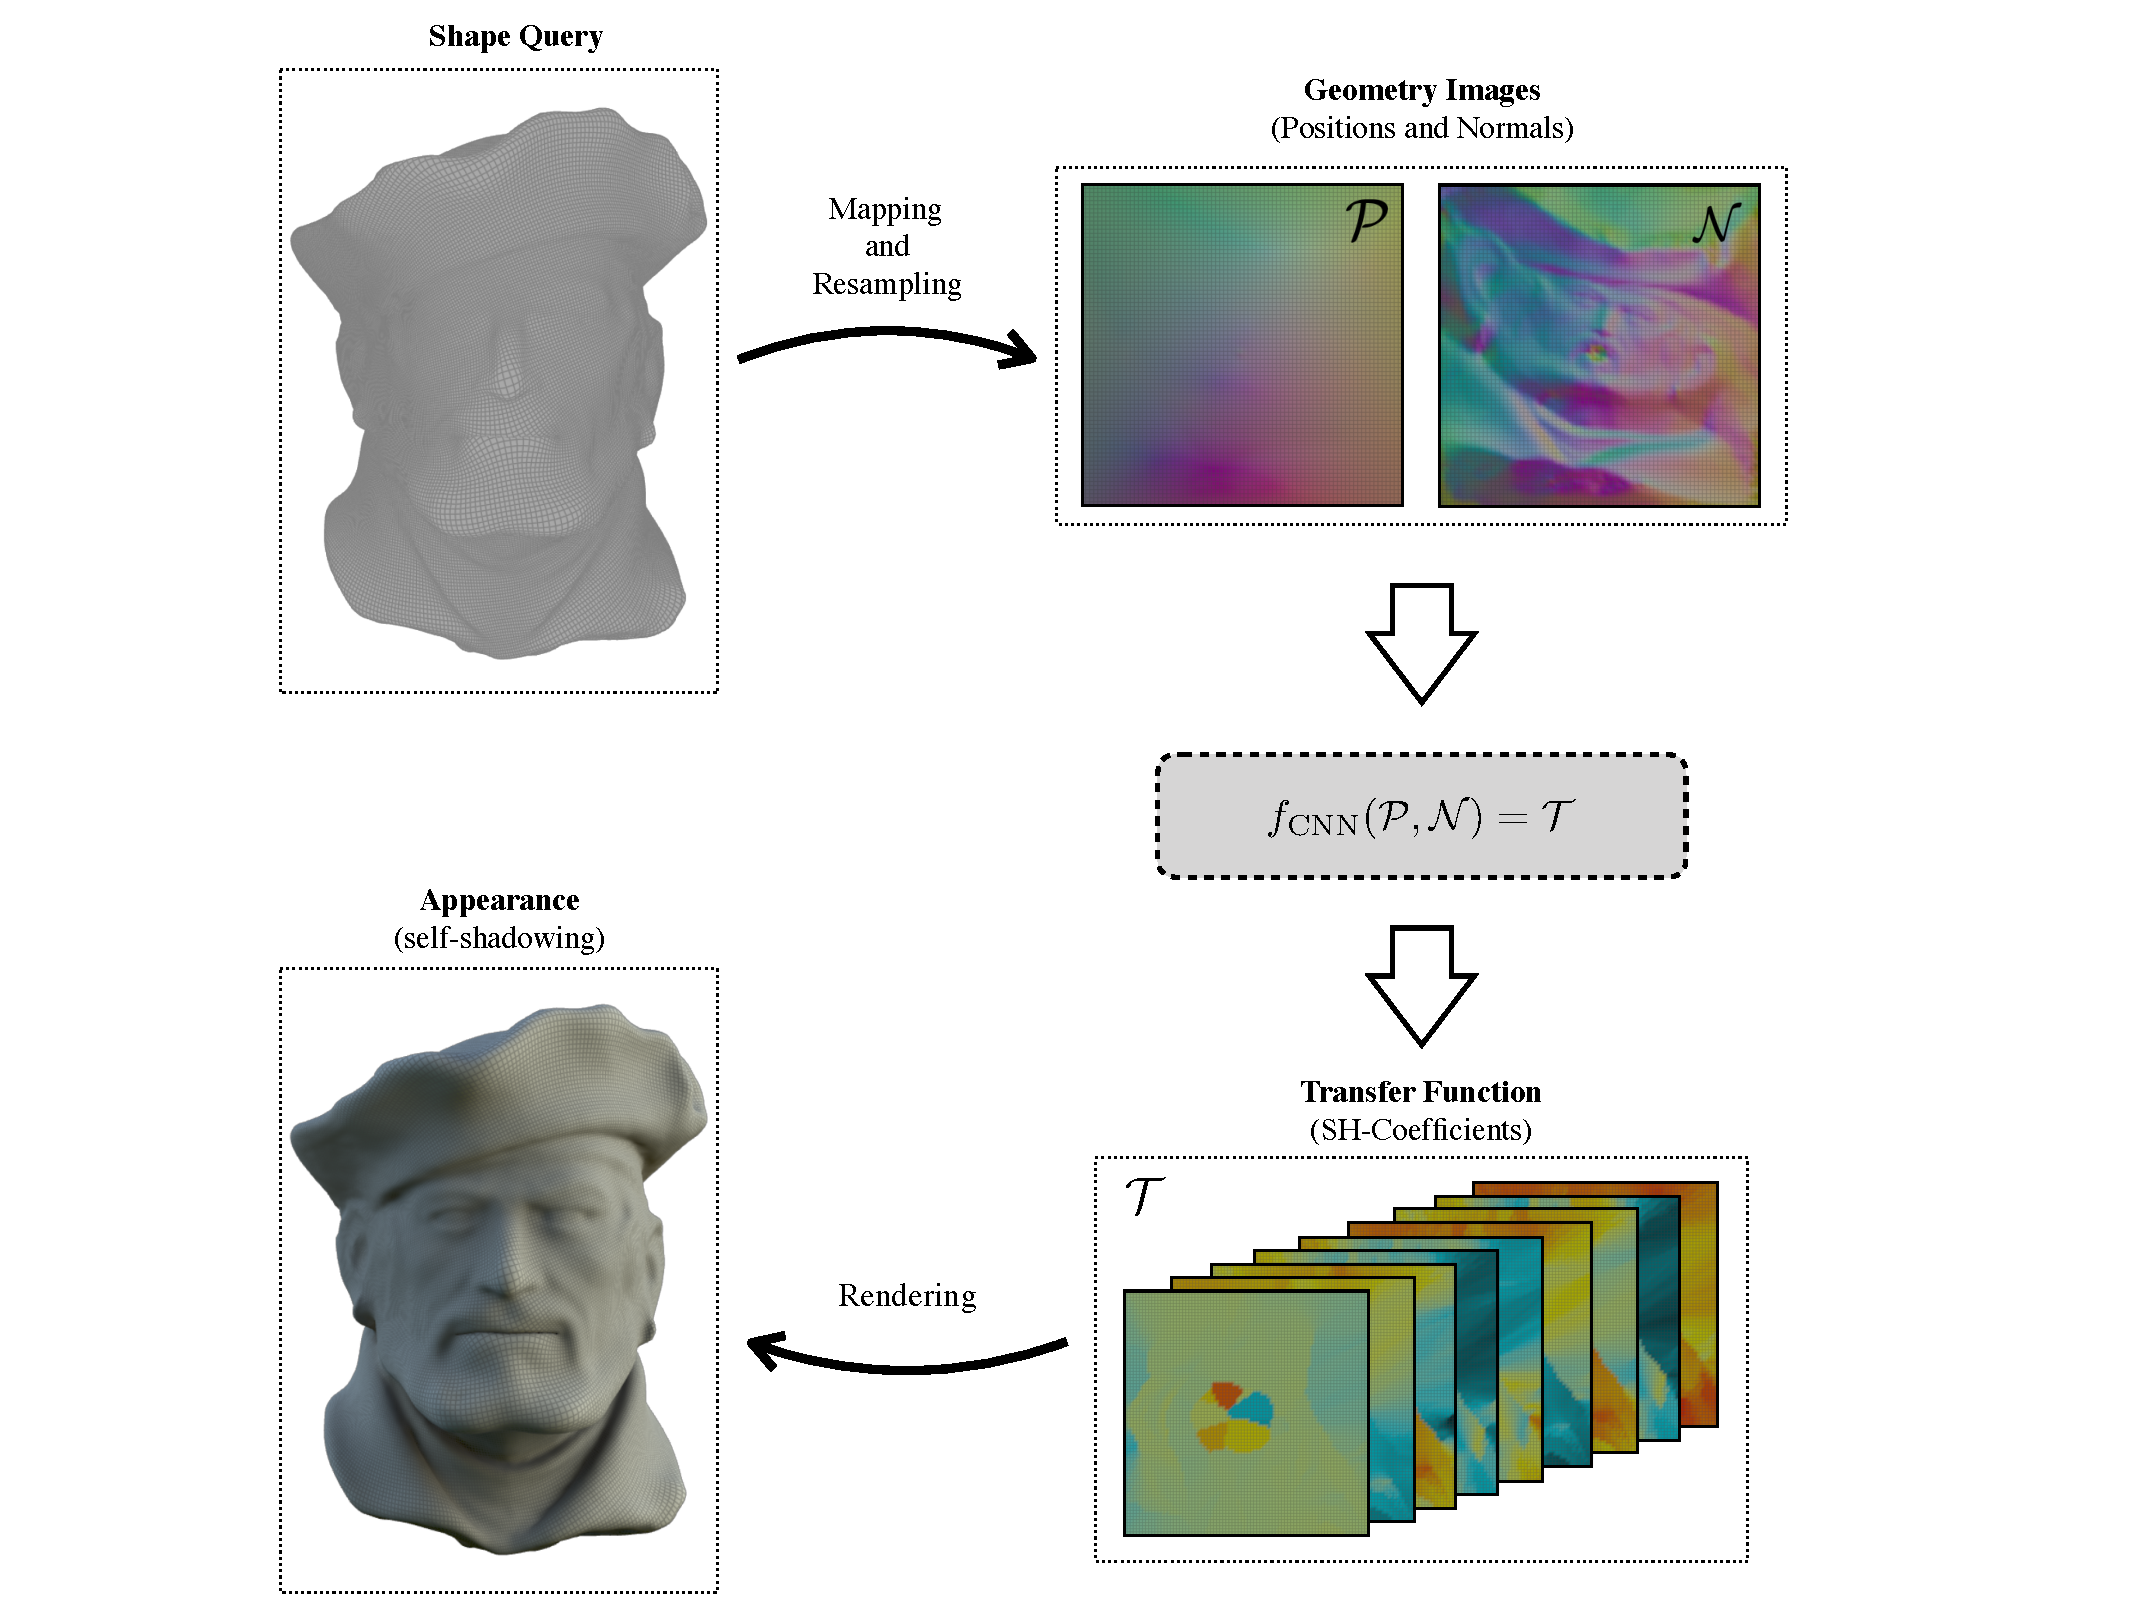
\includegraphics[width=0.5\textwidth]{Figures/Overview_method.pdf}
     \caption{Method Overview}
     \label{Fig: Method_Overview}
\end{figure}
%%%%%%%%%%%%%%%%%%%%%%%%%%%%%%%%%%
% -------------- GEOMETRY IMAGE ----------------- 
%%%%%%%%%%%%%%%%%%%%%%%%%%%%%%%%%%
\subsection{Data: Geometry Images}
We propose learning directly \textbf{on} the object's surface to leverage its underlying shape structure. \textit{Geometry Images} present an intrinsic shape representation on which standard 2D CNNs can be applied \cite{gu2002geometry, sinha2016deep}. 
\\ 
Surfaces with a single boundary (topological disks) are mapped onto a unit square and later discretized (or resampled) into a regular grid of $n \times n$ vertices. 
For simplicity and demonstration purposes, but without loss of generality of our method, we  chose a \textit{Harmonic Map} parametrisation, based on \cite{HarmonicMapping}, for the interior of the 2D-grid. 
\\
\\
The surface information we transform into \textit{Geometry Images} to use as regressor for the CNN are vertex positions $\mathcal{P}$ and normals $\mathcal{N}$. 
\begin{align*}
	\mathcal{P} = \{ P_x, P_y, P_z \} , \quad
	\mathcal{N} = \{ N_x, N_y, N_z \}  
\end{align*}
with  $P_i, N_i \in \mathbb{R}^{n \times n }$ being the position and normal images, respectively, for each coordinate $i \in \{ x,y,z\}$.
\\
\\
We treat each input image of the input set $\{\mathcal{P}, \mathcal{N} \}$ as individual channel. Resulting, our CNN model predicts a corresponding set of \textit{Geometry Images} $\mathcal{T}$,
\begin{align*}
	f_{CNN} :  [\mathcal{P} \times \mathcal{N}] \rightarrow \mathcal{T} 
\end{align*}
consisting of the SH-coefficients of the \textit{Transfer Function} of the input shape, as introduced above (see eq. \ref{Eq: Reduced Rendering Eq}):
\begin{align*}
	\mathcal{T} = \{ t_j \in \mathbb{R}^{n \times n } : j \in \{1,2,...,m\}\} 
\end{align*}
that is, vertex $i$ of image $t_j$ represents the transfer coefficient $j$ of vertex $i$ of the input surface.
\\
Figure \ref{Fig: Method_Overview} illustrates the basic procedure of the method.

\subsection{ Network Architecture and Training}
\subsubsection*{Architecture: } Our network is based on the ResNeXt models introduced in \cite{ResNeXt} (see Figure \ref{Fig: CNN_Architecture}) and has an approximate amount of  11k parameters.
\\
 
\subsubsection*{Training: }
For the training of the network, we generate data synthetically. We produce animations, such as cloth or faces (see examples in section ??) of deforming objects of 500 frames of duration. 
\begin{align*}
&\mathcal{D} = \{  \mathcal{P} , \mathcal{N} , \mathcal{T}\} 
\end{align*}
of position and normal images ($\mathcal{P}= \{ P_x , P_y, P_z \} $  and $\mathcal{N}= \{ N_x , N_y, N_z \} $) are created, where 
\begin{align*}
&P_i,N_i \in \mathbb{R}^{M \times M} ,
\quad
i \in \{x,y,z\}
\end{align*}
As regressand, or ground truth data,  we perform a full self-shadowing integration using ray-casting to calculate the SH-coefficients of the Transfer Function $\mathcal{T}= \{ T_0 , T_1, T_2, T_3..., T_{n^2} \} $ 

\begin{figure}[H]
  \centering
    \includegraphics[width=0.5\textwidth]{Figures/YueLi_network_sketch.pdf}
     \caption{CNN Architecture}
     \label{Fig: CNN_Architecture}
\end{figure}




